%\shorthandoff{:!}

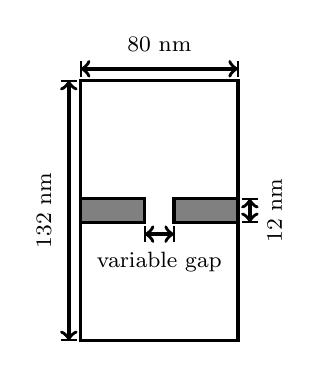
\begin{tikzpicture}[scale=0.025]

%%%%%%%%%%%%%%%%%%%%%%
%%%	 Def géométrie  %%%
%%%%%%%%%%%%%%%%%%%%%%

\def \diacnt{12}
\def \longueur{80}
\def \vspace{2}
\def \lignecote{8}
\def \hauteur{132}
\def \anglearc{111.5}
\def \gap{15}

%%%%%%%%%%%%%%%%%%%%%%
%%%	   Def style    %%%
%%%%%%%%%%%%%%%%%%%%%%

\def \heavy{0.045cm}
\def \light{0.025cm}

%%%%%%%%%%%%%%%%%%%%%%
%%%	    Calculs     %%%
%%%%%%%%%%%%%%%%%%%%%%

\pgfmathsetmacro{\sinangle}{sin(\anglearc)}
\pgfmathsetmacro{\cosangle}{cos(\anglearc)}

%%%%%%%%%%%%%%%%%%%%%%
%%%	    Dessin      %%%
%%%%%%%%%%%%%%%%%%%%%%

\draw[line width=\heavy] (0,0) rectangle (\longueur,\hauteur);
\draw[line width=\heavy, fill=gray] (0,0.5*\hauteur-0.5*\diacnt) rectangle (0.5*\longueur-0.5*\gap,0.5*\hauteur+0.5*\diacnt);
\draw[line width=\heavy, fill=gray] (0.5*\longueur+0.5*\gap,0.5*\hauteur-0.5*\diacnt) rectangle (\longueur,0.5*\hauteur+0.5*\diacnt);


%%%%%%%%%%%%%%%%%%%%%%
%%%	    Cotation    %%%
%%%%%%%%%%%%%%%%%%%%%%

% On dessine la ligne de cote pour l'espace entre les nanotubes
\draw[line width=\light] (0.5*\longueur-0.5*\gap,-\vspace+0.5*\hauteur-0.5*\diacnt) -- + (0,-\lignecote);
\draw[line width=\light] (0.5*\longueur+0.5*\gap,-\vspace+0.5*\hauteur-0.5*\diacnt) -- + (0,-\lignecote);
\draw[<->,line width=\heavy] (0.5*\longueur-0.5*\gap,-\vspace-0.5*\lignecote+0.5*\hauteur-0.5*\diacnt) -- + (\gap,0);

\node[anchor=north] (A) at (0.5*\longueur , -\vspace-\lignecote+0.5*\hauteur-0.5*\diacnt) {\footnotesize variable gap};

% On dessine la ligne de cote pour le diamètre des nanotubes
\draw[line width=\light] (\longueur+\vspace,0.5*\hauteur-0.5*\diacnt) -- + (\lignecote,0);
\draw[line width=\light] (\longueur+\vspace,0.5*\hauteur+0.5*\diacnt) -- + (\lignecote,0);
\draw[<->,line width=\heavy] (\longueur+\vspace+0.5*\lignecote,0.5*\hauteur-0.5*\diacnt) -- + (0,\diacnt);

\node[anchor=north, rotate=90] (B) at (\longueur+\vspace+\lignecote,0.5*\hauteur ) {\footnotesize \diacnt \ nm};

% On dessine la ligne de cote pour la hauteur
\draw[line width=\light] (-\vspace,0) -- + (-\lignecote,0);
\draw[line width=\light] (-\vspace,\hauteur) -- + (-\lignecote,0);
\draw[<->,line width=\heavy] (-\vspace-0.5*\lignecote,0) -- + (0,\hauteur);

\node[anchor=south, rotate=90] (C) at (-\vspace-\lignecote,0.5*\hauteur ) {\footnotesize \hauteur \ nm};

% On dessine la ligne de cote pour le diamètre du modèle
\draw[line width=\light] (0,\hauteur+\vspace) -- + (0,\lignecote);
\draw[line width=\light] (\longueur,\hauteur+\vspace) -- + (0,\lignecote);
\draw[<->,line width=\heavy] (0,\hauteur+\vspace+0.5*\lignecote) -- + (\longueur,0);

\node[anchor=south] (D) at (0.5*\longueur , \hauteur+\vspace+\lignecote) {\footnotesize \longueur \ nm};

%%%%%%%%%%%%%%%%%%%%%%%%%%%%%%%%%%%%%%%%%

\end{tikzpicture}

%\shorthandon{:!}